\documentclass[10pt,twocolumn]{article}


\usepackage[utf8]{inputenc}
\usepackage{abstract}			% L'abstract in cima
\usepackage{geometry}
\usepackage{blindtext}
\usepackage{titlesec}
\usepackage{graphicx}			% Immagini
\usepackage[italian]{babel}		% Italiano
\usepackage[colorlinks=true, linkcolor=black]{hyperref}
\usepackage{amsmath}
\usepackage{booktabs}
\usepackage{tabularx}			% Tabelle fatte bene
\usepackage{caption}			% Captoins per figure
\usepackage{subcaption}		% Subcaptions per figure side by side
\usepackage{siunitx} 			% SI units carini

\DeclareMathOperator\erf{erf} %\erf fa error function

\graphicspath{ {./Images/} }

\geometry{a4paper, top=2cm, bottom=2.5cm, left=2cm, right=2cm}
\setlength{\absleftindent}{3cm}
\setlength{\absrightindent}{3cm}

\title{Studio caratteristico dello scattering Compton}
\author{Jacopo Omodei}
\date{\today}


\begin{document}

\twocolumn[
\maketitle % need full-width title
\begin{onecolabstract}
In questa esperienza è stato studiato sperimentalmente lo scattering Compton di fotoni $\gamma$ emessi da una sorgente di $^{60}$Co. Utilizzando uno scintillatore plastico come bersaglio e un rivelatore NaI(Tl) per la misura dell’energia dei fotoni diffusi, è stata analizzata la dipendenza dell’energia dei fotoni dall’angolo di scattering.
Le posizioni dei picchi energetici sono state stimate tramite fit di likelihood degli spettri acquisiti a diversi angoli, e le incertezze sono state valutate tenendo conto sia degli errori statistici sia dell’errore angolare mediante la tecnica degli errori efficaci. I dati sperimentali sono stati confrontati con il modello teorico di Compton e con una simulazione Monte Carlo, utilizzata per stimare gli effetti geometrici del set-up.
I risultati mostrano un accordo qualitativo con le previsioni teoriche, evidenziando tuttavia la presenza di contributi sistematici riconducibili alla risoluzione energetica del rivelatore, alla calibrazione in energia e alla stabilità del guadagno dei fotomoltiplicatori nel tempo.
\end{onecolabstract}
]

\tableofcontents
\section{Introduzione}
\label{sec:intro}

Lo scopo dell’esperienza è la verifica sperimentale della distribuzione energetica e della dipendenza angolare dei fotoni diffusi nel processo di scattering Compton. 

Lo scopo di questa esperienza di laboratorio è verificare la presenza dell'effetto Compton per una sorgente radioattiva di cobalto 60, che emette due fotoni di energia pari a $\SI{1.17}{MeV}$ e $\SI{1.33}{MeV}$ tramite $\beta$\textit{-decay}. Nello studio di questo effetto, la sorgente è stata posizionata davanti a una targhetta di materiale scintillante plastico, e i fotoni emessi dal cobalto (dopo essere passati attraverso un collimatore di piombo per ridurre la divergenza angolare del fascio) colpiscono il bersaglio di materiale scintillante; una parte di essi interagisce tramite l'effetto Compton, cedendo una frazione della propria energia al materiale e variando la direzione di volo. Un rivelatore a cristallo di NaI, vincolato a muoversi su una guida circolare a una distanza fissa dal bersaglio, raccoglie una porzione dei fotoni diffusi e ne misura l'energia. Lo studio consiste nel variare l'angolo del rivelatore cristallino e nel registrare la dipendenza dell'energia dei fotoni rilevati dall'angolo di scattering nel bersaglio, con l'obiettivo di ritrovare l'andamento previsto dall'effetto Compton:
\begin{equation}
E^\prime = \frac{E_0}{1+\left(\frac{E_0}{m_ec^2}\right)\left(1-\cos\Phi\right)}
\label{eq:Compton_formula}
\end{equation}

L'idea dell'esperimento, quindi, è misurare la distribuzione di energia dei fotoni assorbiti nel rivelatore per diversi angoli di scattering.


\section{Apparato sperimentale}
\label{sec:apparatus}

L'apparato sperimentale è composto da una sorgente radioattiva di $^{60}$Co collocata all'interno di una schermatura in piombo. La schermatura presenta un foro cilindrico nel quale è inserito un collimatore con raggio interno di \SI{1}{cm} e lunghezza di \SI{11}{cm}. Il collimatore consente di selezionare un fascio di fotoni $\gamma$ con una divergenza angolare massima rispetto al proprio asse pari a

\begin{equation}
\alpha_{max} = \arctan\left(\frac{2\cdot r_{coll}}{L_{coll}}\right)\simeq 10^\circ
\label{eq:div_coll}
\end{equation}

A \SI{2}{cm} dal collimatore è posizionato uno scintillatore plastico di forma parallelepipeda rettangolare, spesso \SI{3}{cm}, accoppiato a un fotomoltiplicatore (\textit{PMT1}). Tale rivelatore funge da bersaglio per il processo di scattering Compton e consente anche la rivelazione dell'elettrone diffuso, che verrà utilizzata successivamente per implementare un segnale di coincidenza, permettendo così di ridurre il rumore dovuto alle coincidenze accidentali. 

Il fotone diffuso viaggia nell'aria prima di incidere su un cristallo di ioduro di sodio drogato con tallio (NaI(Tl)), con altezza e diametro uguali e pari a \SI{5.08}{cm}. Questo cristallo è accoppiato a un secondo fotomoltiplicatore (\textit{PMT2}), che insieme al cristallo costituisce un secondo rivelatore. Il rivelatore è montato su una guida metallica che consente di variare l'angolo tra il bersaglio di plastica (che funge da origine attorno a cui ruota il secondo rivelatore) e il cristallo; tramite un goniometro è inoltre possibile misurare l'angolo compreso tra i due rivelatori. Per tutte le misure si è deciso di mantenere il cristallo a una distanza di \SI{38}{cm} dal plastico (misurata tra il centro del plastico e la faccia più vicina del cristallo), che risulta essere la distanza massima consentita dalla guida metallica.

\subsection{Acquisizione del segnale}
\label{subsec:as}

\begin{figure*}[ht!]
\captionsetup{width=.8\linewidth}
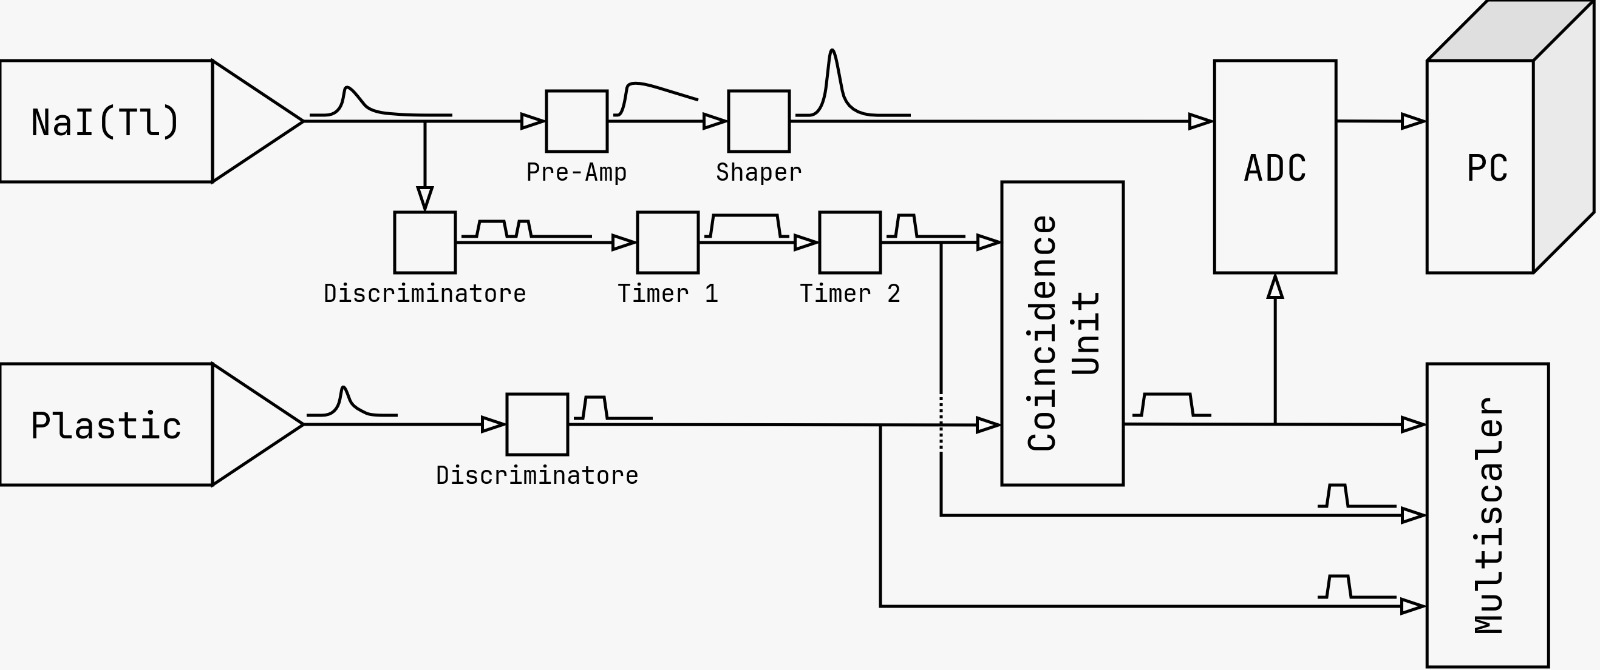
\includegraphics[width=0.8\linewidth]{Catena.jpeg}
\centering
\caption{Schema riassuntivo degli elementi della catena di acquisizione ed elaborazione del segnale}
\label{fig:catena}
\end{figure*}

Lo scopo dell'esperimento è misurare l'energia dei fotoni che hanno subito uno scattering Compton nello scintillatore plastico al variare dell'angolo di scattering. 
Per misurare l'energia residua di un fotone che ha subito uno scattering Compton si utilizza un fotomoltiplicatore accoppiato allo ioduro di sodio, che fornisce un segnale analogico proporzionale alla quantità di energia depositata (a sua volta proporzionale al numero di fotoni prodotti nel materiale scintillante). Questo segnale viene inviato a un preamplificatore di carica (un integratore con costante di tempo pari a \SI{60}{\mu s}) e, per evitare fenomeni di pile-up e migliorare il rapporto segnale-rumore, la forma d'onda viene modellata mediante uno \textit{shaper} (\textit{Ortec 435}), derivando il segnale integrato. Il segnale, la cui ampiezza rimane proporzionale a quella iniziale, viene quindi inviato all'\textit{ADC} (\textit{CAEN N957}, \textit{MCA} da 8K canali, risoluzione nominale di 13 bit e range dinamico analogico 0–10~V), che costruisce lo spettro di energia in unità arbitrarie, con valore massimo pari a 8192. 

Il segnale acquisito è dominato da rumore accidentale, dovuto in parte all'agitazione termica del cristallo di NaI, a fotoni esterni e ai raggi cosmici, oltre ad altri contributi. Per selezionare solo gli eventi in cui è effettivamente avvenuto uno scattering Compton, è stata implementata una coincidenza tra il segnale rilasciato dal primo fotomoltiplicatore e quello del secondo. Più precisamente, il segnale non amplificato del \textit{PMT2} viene inviato a un discriminatore con soglia pari a $\sim \SI{-16}{mV}$ e successivamente fatto passare attraverso due \textit{timer} consecutivi: il primo impone un tempo morto di \SI{1.4}{\mu s}, mentre il secondo genera un segnale logico della durata di \SI{44.2}{ns}. Lo scopo di questi due \textit{timer} è contare solo il primo superamento della soglia del discriminatore e generare successivamente un segnale di breve durata da utilizzare nella coincidenza. 

Il segnale del \textit{PMT1}, invece, attraversa unicamente un discriminatore con soglia pari a $\sim \SI{-16}{mV}$, generando un segnale logico della durata di \SI{73}{ns}. Dopo aver ritardato opportunamente il segnale del primo fotomoltiplicatore tramite una serie di cavi coassiali di lunghezza adeguata, i due segnali logici vengono inviati a un'unità di coincidenza, che produce un segnale logico utilizzato per discriminare gli eventi con deposito di energia sia nel plastico sia nello ioduro. Tale segnale viene utilizzato come \textit{trigger} dell'\textit{ADC}, consentendo di selezionare esclusivamente gli eventi di interesse. 

Per misurare il \textit{rate} in funzione dell'angolo dei fotoni scatterati si utilizza un \textit{multiscaler} a 8 canali. I suoi ingressi includono il segnale in uscita dall'unità di coincidenza (assunto come numero di eventi di scattering misurati) e i due segnali logici dei \textit{PMT} (che rappresentano il conteggio delle coincidenze accidentali sommate agli eventi di scattering per ciascun fotomoltiplicatore). Una rappresentazione schematica della catena di acquisizione è riportata in figura~\ref{fig:catena}.


\subsection{Alimentazione dei PMT}
\label{subsec:alimentazione}

Per stabilire l'alimentazione, e quindi i punti di lavoro, dei fotomoltiplicatori, è stato inizialmente utilizzato il \textit{PMT2} in modalità singola, senza la catena di coincidenza descritta in sezione~\ref{subsec:as}. Ponendo il cristallo davanti alla sorgente ($\Phi = 0$), è stato acquisito lo spettro del cobalto al variare dell'alimentazione del fotomoltiplicatore. Naturalmente, questa misura contiene un contributo significativo di rumore; tuttavia, il \textit{rate} del cobalto risulta sufficientemente elevato da rendere distinguibili due picchi al di sopra del \textit{background} rumoroso. 

\begin{figure}[ht!]
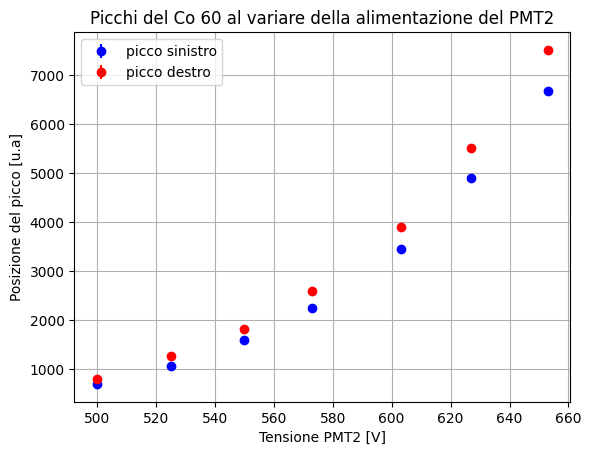
\includegraphics[width=0.9\linewidth]{pos_picchi_pmt2.png}
\centering
\caption{Posizione dei picchi del $^{60}$Co, in unità arbitrarie di canale, in funzione dell'alimentazione del \textit{PMT2}}
\label{fig:pmt2_picchi}
\end{figure}

In parallelo, il segnale diretto del \textit{PMT2} e quello amplificato sono stati visualizzati su un oscilloscopio con impedenza di ingresso pari a \SI{1}{M\Omega}. La tensione di alimentazione è stata fissata a \SI{630}{V}, scelta in modo tale da far corrispondere un fotone di energia pari a \SI{1}{MeV} a un segnale di ampiezza $\sim$\SI{-20}{mV}, così da superare la soglia di discriminazione precedentemente impostata a \SI{-16}{mV}. Contestualmente, è stato verificato che il segnale amplificato non andasse in saturazione e che lo spettro acquisito consentisse di visualizzare due picchi chiari e ben distinti, lontani dalla regione di saturazione. Come mostrato in figura~\ref{fig:pmt2_picchi}, alimentazioni più elevate producono una maggiore separazione tra i picchi, caratteristica necessaria nello svolgimento dell'esperienza per distinguere i due fotoni emessi. Questo valore di alimentazione è stato quindi utilizzato per il resto dell'esperienza per il secondo fotomoltiplicatore.

\begin{figure}[ht!]
\includegraphics[width=0.9\linewidth]{telescope.jpeg}
\centering
\caption{Set-up utilizzato per configurare l'alimentazione del \textit{PMT1}}
\label{fig:telescope}
\end{figure}

Per determinare l’alimentazione del \textit{PMT1}, i due scintillatori sono stati montati su un supporto differente rispetto a quello descritto in precedenza, in modo da poterli utilizzare come un piccolo telescopio per raggi cosmici, riportato in figura~\ref{fig:telescope}. In questa configurazione, sfruttando il \textit{trigger} sulle coincidenze dei due segnali, il sistema è stato utilizzato per determinare un punto di lavoro adeguato del \textit{PMT1}. 

Si è assunto che i raggi cosmici perdano in media \SI[per-mode = fraction]{1}{\MeV\per\cm} all'interno dello scintillatore plastico (densità media $\sim$\SI[per-mode = fraction]{1}{\g\per\cm^3}). Assumendo inoltre che i raggi cosmici si trovino mediamente nella regione di \textit{MIP} (\textit{Minimum Ionization Point}), e quindi abbiano un'energia di circa \SI{1.5}{\MeV}, e considerando che lo scintillatore ha uno spessore di \SI{2}{cm}, l'energia depositata risulta essere di circa \SI{3}{\MeV}. Volendo impostare una soglia di \SI{-20}{mV} per un deposito di energia di \SI{100}{keV}, e quindi un segnale di circa \SI{-600}{mV} per \SI{3}{MeV}, è stata selezionata una tensione di alimentazione pari a \SI{1830}{V}. Questo valore di soglia è stato mantenuto per l'intera durata dell'esperienza.
\section{Elaborazione del segnale}
\label{sec:elab}

Per misurare lo spettro dell'energia depositata dai fotoni nel cristallo scintillatore a un angolo $\Phi$, si utilizza l'interfaccia \textit{software} dell'\textit{ADC} sul computer e si acquisiscono gli istogrammi degli spettri di energia misurati in unità arbitrarie di canale. Il segnale misurato è linearmente proporzionale alla quantità di energia depositata all'interno del cristallo. Inoltre, l'\textit{ADC} viene operato in modalità di \textit{trigger} esterno, acquisendo esclusivamente gli eventi che soddisfano la condizione di coincidenza tra i due fotomoltiplicatori. 

\subsection{Calibrazione}
\label{subsec:calibrazione}
 
Poiché gli spettri di energia sono riportati in unità di canale, lo strumento è stato calibrato per determinare una relazione che associasse le misure in canali a misure di energia in keV. A tal fine sono state utilizzate diverse sorgenti radioattive, oltre alla sorgente principale di $^{60}$Co. Le sorgenti impiegate e le corrispondenti energie dei picchi a maggiore probabilità sono riportate in tabella~\ref{tab:sorgenti}.

\begin{table}[ht]
\centering
\begin{tabular}{ll} 
\hline
\noalign{\smallskip}
\textbf{Sorgente} & \textbf{Energia del picco [keV]} \\ [0.5ex] 
\hline
\noalign{\smallskip}
$^{241}$Am 	& 59.5 \\
$^{22}$Na   	& 511.0 \\
$^{137}$Cs  	& 661.7 \\
$^{60}$Co    	& 1173.2, 1332.5 \\
\hline
\end{tabular}
\caption{Sorgenti radioattive utilizzate per la calibrazione canali--energia}
\label{tab:sorgenti}
\end{table}

Mediante l'utilizzo di una montatura dedicata che permette di allineare una sorgente radioattiva con il cristallo, è stato acquisito lo spettro di ciascuna sorgente in modalità singola, quindi senza le coincidenze con il plastico. In modo analogo a quanto descritto in sezione~\ref{subsec:alimentazione}, gli spettri sono stati acquisiti fino a quando i principali picchi di emissione risultavano ben distinguibili dal rumore di fondo. 

La posizione dei picchi è stata determinata in unità di canale dell'\textit{ADC} mediante un fit con un modello costituito dalla somma di un picco gaussiano e di un fondo esponenziale, applicato in una finestra ristretta attorno al picco stesso. I parametri iniziali del fit e l'estensione della finestra sono stati scelti manualmente sulla base della forma dello spettro. Questo procedimento consente di stimare la posizione del picco con la relativa incertezza; nel caso del $^{60}$Co, sono stati determinati entrambi i picchi di emissione, utilizzando un modello a doppia gaussiana sommato a un fondo esponenziale. 

\begin{figure*}[htp]
    \centering
    \begin{subfigure}[b]{0.3\textwidth}
        \centering
        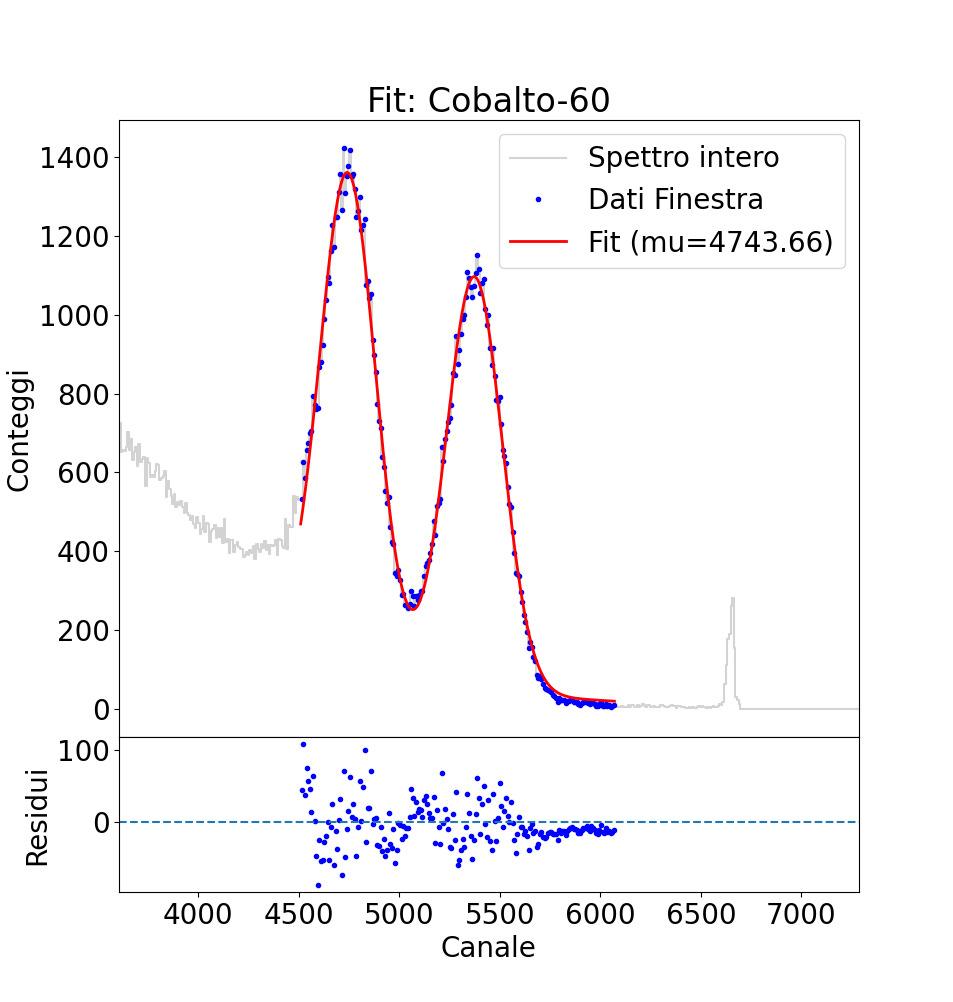
\includegraphics[width=\textwidth]{calCo.jpeg}
        \caption{Fit con doppia gaussiana e fondo esponenziale per $^{60}$Co.}
    \end{subfigure}
    \hfill
    \begin{subfigure}[b]{0.3\textwidth}
        \centering
        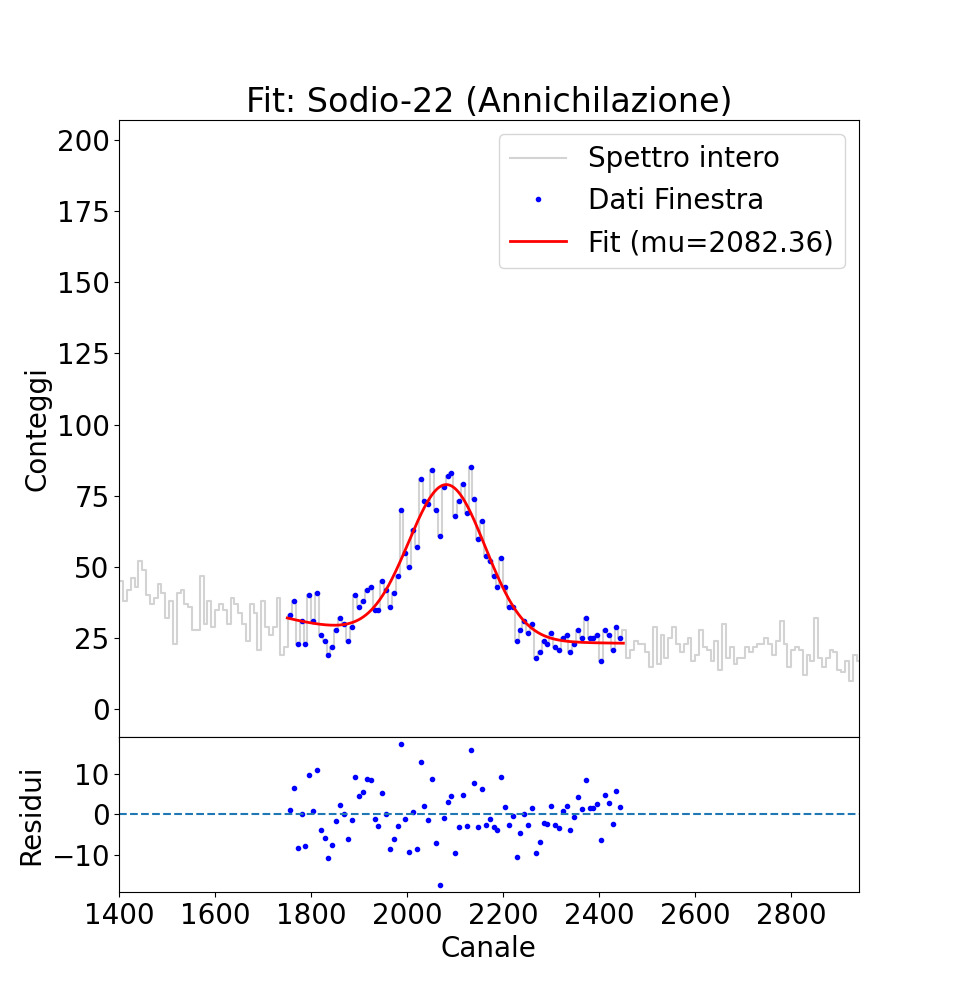
\includegraphics[width=\textwidth]{calNa.jpeg}
        \caption{Fit con singola gaussiana e fondo esponenziale per $^{22}$Na.}
    \end{subfigure}
    \hfill
    \begin{subfigure}[b]{0.3\textwidth}
        \centering
        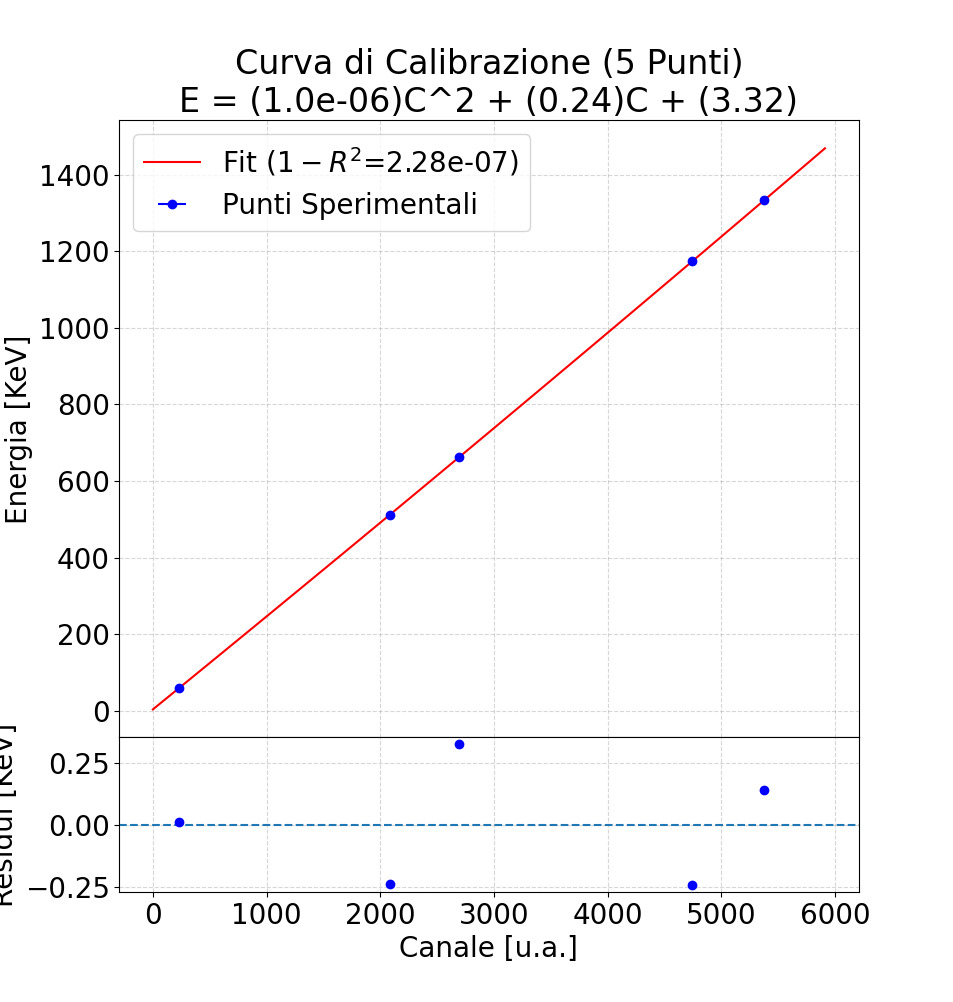
\includegraphics[width=\textwidth]{curvacal.jpeg}
        \caption{Curva di calibrazione, polinomio di secondo grado.}
    \end{subfigure}
    
    \caption{Caratterizzazione e calibrazione in energia del rivelatore NaI(Tl) tramite sorgenti standard.}
    \label{fig:calibrazioni}
\end{figure*}

Conoscendo l'energia teorica dei picchi e misurando il canale corrispondente mediante questa procedura, la relazione tra energia e canale è stata determinata utilizzando un polinomio di secondo grado nei canali, al fine di includere eventuali contributi non lineari della catena di acquisizione. Due esempi di fit, insieme ad una curva di calibrazione vengono riportati in figura \ref{fig:calibrazioni}.

A ogni accensione dell'apparato, e quindi a ogni giornata di presa dati, l'intero processo di calibrazione è stato ripetuto, in modo da compensare eventuali variazioni di guadagno dovute a fluttuazioni nelle tensioni di alimentazione dei fotomoltiplicatori o a variazioni delle condizioni ambientali. In questo modo, a ciascuna acquisizione corrisponde una curva di calibrazione dedicata, che consente di convertire le misure da canali a keV.
\subsection{Analisi del rate al variare dell'angolo}
\label{subsec:rate}

Al fine di allocare un tempo di acquisizione adeguato a ciascuna misura, è stata effettuata una misura del \textit{rate} degli eventi di coincidenza in funzione dell'angolo di scattering $\Phi$. Utilizzando il \textit{multiscaler}, come discusso in sezione~\ref{subsec:as}, sono stati conteggiati il numero di singoli per ciascun fotomoltiplicatore e il numero di coincidenze al variare dell'angolo del cristallo $\Phi$. In figura~\ref{fig:rate} sono riportati i risultati sperimentali del numero di coincidenze in funzione dell'angolo, insieme alla stima del contributo dovuto alle coincidenze accidentali. 

\begin{figure}[ht!]
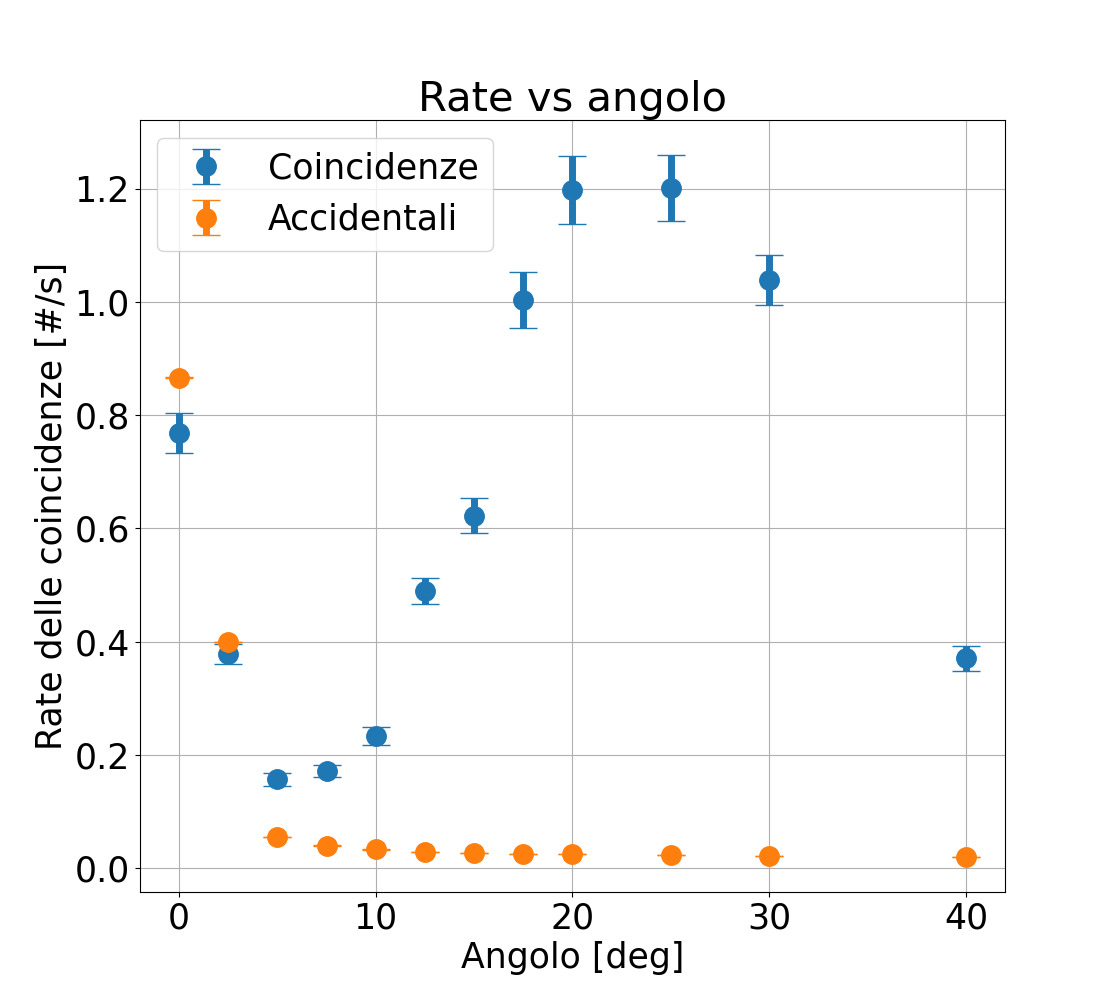
\includegraphics[width=0.9\linewidth]{rate.jpeg}
\centering
\caption{\textit{Rate} delle coincidenze in funzione dell’angolo, insieme alla stima del \textit{rate} delle coincidenze accidentali. Gli errori sui \textit{rate} sono stati assunti come poissoniani sui conteggi ($\sigma_R = \frac{\sqrt{N}}{\Delta t}$).}
\label{fig:rate}
\end{figure}

Per stimare il \textit{rate} di coincidenze accidentali è stata utilizzata la relazione:
\begin{equation}
R_{acc} \simeq R_1 \cdot R_2 \left( \Delta t_1 + \Delta t_2 - 2\tau \right),
\label{eq:coincidenze_acc}
\end{equation}
dove $R_1$ e $R_2$ rappresentano i \textit{rate} di conteggio dei singoli rivelatori, espressi in conteggi al secondo (ossia il numero riportato dal \textit{multiscaler} diviso il tempo di acquisizione in secondi). Le quantità $\Delta t_1$ e $\Delta t_2$ sono le larghezze temporali dei segnali logici in ingresso all'unità di coincidenza (\SI{73}{ns} e \SI{44}{ns}, rispettivamente), mentre $\tau$ è il tempo minimo di sovrapposizione richiesto affinché si verifichi una coincidenza (\SI{2}{ns}). 

Dal punto di vista teorico ci si aspetta un andamento del \textit{rate} monotono decrescente all'aumentare dell'angolo di scattering, in accordo con la sezione d'urto differenziale di Klein--Nishina. Tuttavia, si osserva che a piccoli angoli il \textit{rate} è completamente dominato dal contributo del fascio diretto e dagli eventi accidentali; inoltre, le misure mostrano chiaramente un massimo locale nella regione intorno a $22.5^\circ$. Questo comportamento è attribuibile al fatto che la soglia del discriminatore sul rivelatore plastico seleziona gli eventi di scattering a bassi angoli: se un fotone subisce uno scattering con un angolo di deflessione troppo piccolo, non deposita sufficiente energia nel plastico per superare la soglia del discriminatore e, di conseguenza, l'evento non genera una coincidenza. 

Questo effetto porterà, nelle analisi successive, a una sottostima dell'energia dei picchi per piccoli angoli, poiché i fotoni rivelati saranno prevalentemente quelli che subiscono scattering a angoli maggiori e che, per ragioni geometriche, riescono comunque a raggiungere il rivelatore di NaI. 

Ciononostante, questa misura consente di ottimizzare la distribuzione dei tempi di acquisizione nelle misure successive, pianificando le sessioni di laboratorio in modo da bilanciare il numero di angoli investigati con la statistica disponibile per ciascuna misura.
\section{Acquisizione e analisi dei dati}
\label{sec:analisi}

Il rivelatore è stato posizionato a diversi angoli di scattering, coprendo un intervallo compreso tra $0^\circ$ e $40^\circ$ con incrementi costanti di $5^\circ$. Le misure spettrali sono state effettuate rispettando i tempi definiti dallo scan preliminare discusso nella sezione precedente, al fine di accumulare una statistica significativa per ciascuna configurazione. Dopo aver calibrato gli strumenti, il set-up è stato riportato nella configurazione ottimale (descritta in sezione~\ref{sec:apparatus}) e lo spettro è stato acquisito utilizzando il \textit{trigger}, come discusso in precedenza. Gli spettri sono stati successivamente scaricati e convertiti, tramite la funzione di calibrazione del giorno, in spettri di energia espressi in keV. 

Per angoli piccoli (inferiori a $30^\circ$) si osserva chiaramente la presenza di una ``spalla'' a bassa energia, dovuta al fatto che non tutti i fotoni vengono completamente assorbiti per effetto fotoelettrico all'interno del cristallo. In alcuni casi, infatti, i fotoni subiscono un numero arbitrario di scattering Compton nel cristallo, depositando solo una frazione della loro energia prima di uscire dal materiale. Tali eventi risultano indistinguibili da fotoni di energia inferiore che vengono invece completamente assorbiti nel rivelatore. Per questo motivo è stata fissata una soglia di discriminazione sul secondo fotomoltiplicatore, al fine di eliminare gli eventi che non rilasciano un'energia sufficiente a garantire l'assorbimento completo. Tuttavia, tale soglia è stata scelta in modo da non escludere gli eventi a grandi angoli, per i quali i fotoni di interesse possiedono, a causa dello scattering Compton avvenuto nel plastico, un'energia inferiore rispetto a quelli a piccoli angoli. Di conseguenza, per valori piccoli di $\Phi$ si osserva la presenza della ``spalla Compton'', che tende a scomparire all'aumentare dell'angolo di scattering.

\begin{figure*}[htp]
    \centering
    \begin{subfigure}[b]{0.3\textwidth}
        \centering
        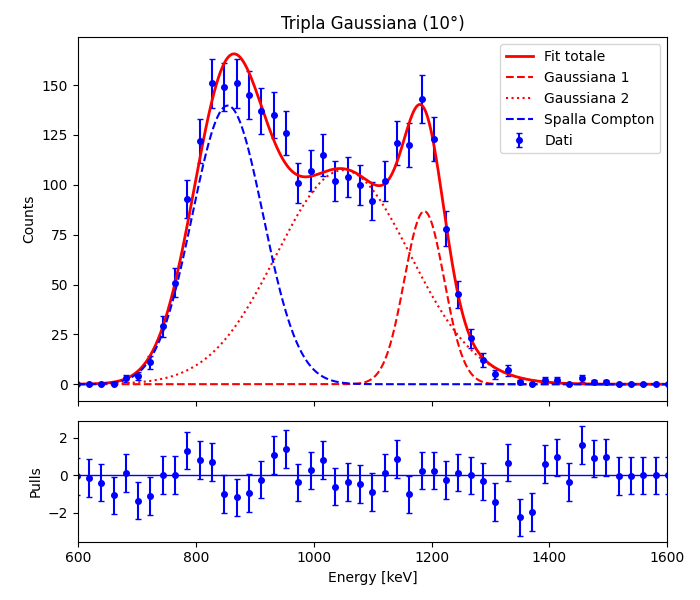
\includegraphics[width=\textwidth]{10deg.png}
        \caption{Fit con tripla gaussiana per piccoli angoli, dove la spalla Compton assume la forma di un terzo picco.}
    \end{subfigure}
    \hfill
    \begin{subfigure}[b]{0.3\textwidth}
        \centering
        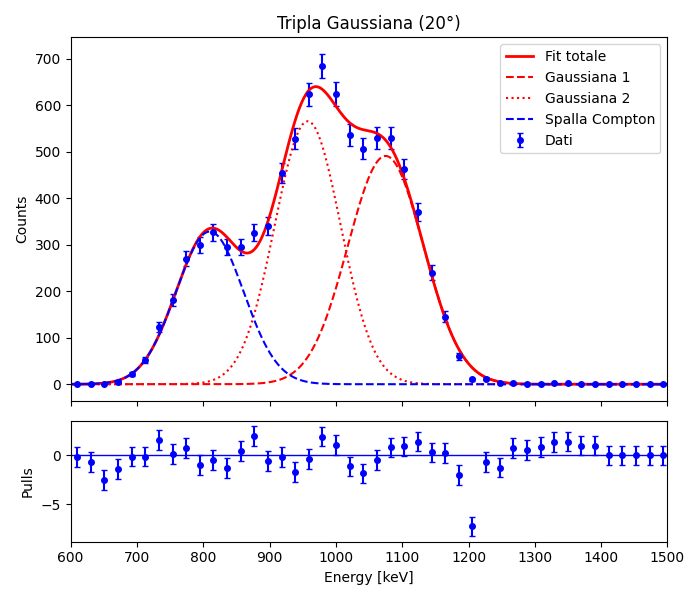
\includegraphics[width=\textwidth]{20deg.png}
        \caption{Fit con tripla gaussiana, in cui la spalla Compton inizia a diminuire in ampiezza grazie all'effetto del discriminatore.}
    \end{subfigure}
    \hfill
    \begin{subfigure}[b]{0.3\textwidth}
        \centering
        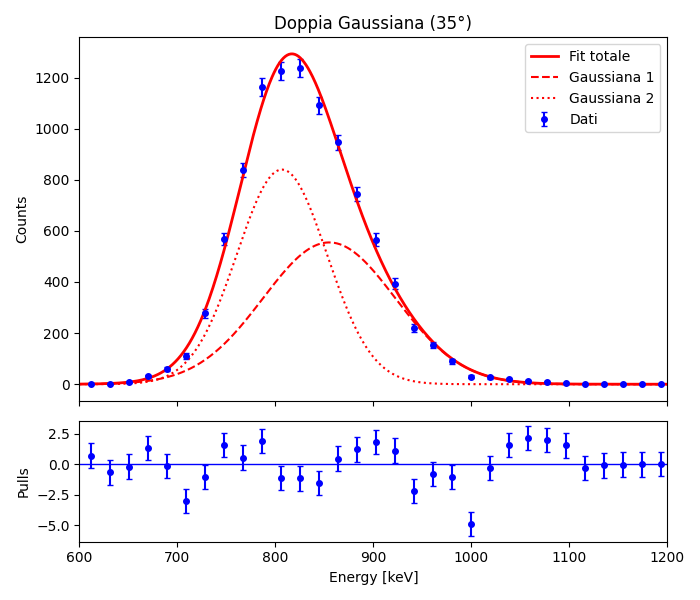
\includegraphics[width=\textwidth]{35deg.png}
        \caption{Fit con due gaussiane, in cui la spalla Compton non è più presente e i due picchi iniziano a sovrapporsi.}
    \end{subfigure}
    
    \caption{Esempi di fit gaussiani utilizzati per determinare la posizione dei picchi a diversi angoli di posizionamento del cristallo. Si osserva l'evoluzione dell'ampiezza e della forma della spalla Compton all'aumentare di $\Phi$.}
    \label{fig:fits}
\end{figure*}

Per identificare correttamente i centroidi dei picchi, l’analisi è stata condotta mediante un \textit{fit di likelihood} sui bin (ridimensionati da 8192 a 100) utilizzando un modello costituito dalla somma di tre gaussiane all'interno della regione di interesse fino a $25^\circ$, dove la spalla Compton risulta ancora visibile. Si noti che l’utilizzo di una gaussiana per descrivere la spalla Compton rappresenta un’approssimazione, poiché la distribuzione fisica sottostante ha una forma differente; tuttavia, in assenza di una parametrizzazione analitica più accurata, questo approccio si è dimostrato il più robusto per garantire la convergenza del fit. All’aumentare dell’angolo, in particolare oltre i $30^\circ$, lo spostamento energetico porta la spalla Compton a scendere al di sotto della soglia di discriminazione del cristallo NaI, rendendola di fatto non osservabile. Per questo motivo, in tale regime il modello è stato semplificato utilizzando soltanto due gaussiane. Un confronto tra i risultati dei fit nelle due diverse condizioni è riportato in figura~\ref{fig:fits}, dove sono mostrati alcuni esempi per differenti angoli di scattering.

\subsection{Stima degli errori}
\label{subsec:errori}

L'incertezza associata alla misura dell'energia corrisponde all'errore standard sui parametri restituito dalla procedura di fit di likelihood. I risultati completi sono riportati in tabella \ref{tab:err}.

\begin{table}[ht]
\centering
\begin{tabular}{ccc} 
\hline
\noalign{\smallskip}
Angolo & $\mu_1$ & $\mu_2$ \\ [0.5ex] 
\hline
\noalign{\smallskip}
$0^\circ$ 	& $1331\pm1$ 	& $1164\pm1$ \\
$10^\circ$ 	& $1222\pm3$ 	& $1081\pm3$ \\
$15^\circ$ 	& $1196\pm2$ 	& $1047\pm3$ \\
$20^\circ$ 	& $1111\pm2$ 	& $988\pm2$ \\
$25^\circ$ 	& $1046\pm1$ 	& $938\pm3$ \\
$30^\circ$ 	& $928\pm2$ 	& $869\pm3$ \\
$35^\circ$ 	& $870\pm6$ 	& $822\pm3$ \\
$40^\circ$ 	& $923\pm3$ 	& $823\pm1$ \\
\hline
\end{tabular}
\caption{Posizione dei picchi dei fotoni stimata tramite fit per i vari angoli di scattering}
\label{tab:err}
\end{table}

La stima dell'errore sull'angolo di scattering deriva invece dalla sensibilità del goniometro, che abbiamo assunto avere una distribuzione uniforme di larghezza $2.5^\circ$. Di conseguenza, l'errore sull'angolo è stato posto pari a
\[
\sigma_\Phi = \frac{2.5^\circ}{\sqrt{12}} \simeq 0.7^\circ
\]
per ogni misura.

Abbiamo inoltre verificato che l'incertezza sull'angolo dovuta all'accettanza geometrica del cristallo fosse trascurabile tramite l'utilizzo di una simulazione Monte Carlo, discussa nell'appendice \ref{app:MC}. L'ordine di grandezza dell'errore sull'angolo medio di scattering dei fotoni incidenti sul cristallo, come stimato dalla simulazione\footnote{Abbiamo studiato la distribuzione dell'angolo di scattering all'interno del bersaglio plastico per tutti i fotoni che raggiungono il cristallo e calcolato l'errore sulla media di tale distribuzione.}, risulta pari a
\[
\frac{5^\circ}{\sqrt{N}} \sim 10^{-3}\,^\circ,
\]
e quindi del tutto trascurabile rispetto alla sensibilità del goniometro.

Abbiamo quindi calcolato gli errori efficaci sugli angoli per poterli confrontare con gli errori sulle posizioni dei picchi, utilizzando la relazione
\begin{equation}
\sigma_{\Phi_{\text{eff}}} = \sigma_\Phi \cdot \left|\frac{\mathrm{d} E_{E_0}^\prime(\Phi)}{\mathrm{d} \Phi}\right|,
\label{eq:phi_eff}
\end{equation}
dove $E_{E_0}^\prime(\Phi)$ è l'espressione (\ref{eq:Compton_formula}) del modello di Compton che vogliamo verificare. I valori ottenuti sono riportati in tabella \ref{tab:err_eff}. Come si osserva, tali contributi risultano maggiori degli errori sulle posizioni dei picchi e non possono quindi essere trascurati; abbiamo pertanto deciso di sommarli in quadratura agli errori statistici, come previsto dalla tecnica degli errori efficaci.

\begin{table}[ht]
\centering
\begin{tabular}{ccc} 
\hline
\noalign{\smallskip}
Angolo & ${\sigma}_{\Phi_{\text{eff},1}}$ & ${\sigma}_{\Phi_{\text{eff},2}}$ \\ [0.5ex] 
\hline
\noalign{\smallskip}
$0^\circ$ 	& $0.0$ 		& $0.0$ \\
$10^\circ$ 	& $7.0$ 		& $5.5$ \\
$15^\circ$ 	& $9.5$ 		& $7.6$ \\
$20^\circ$ 	& $11.2$ 		& $8.9$ \\
$25^\circ$ 	& $11.9$ 		& $9.7$ \\
$30^\circ$ 	& $12.0$ 		& $9.9$ \\
$35^\circ$ 	& $11.6$ 		& $9.7$ \\
$40^\circ$ 	& $10.8$ 		& $9.2$ \\
\hline
\end{tabular}
\caption{Errori efficaci associati all'incertezza sull'angolo di scattering}
\label{tab:err_eff}
\end{table}

\section{Confronto dati e modello teorico}
\label{sec:confronto}

Per verificare la relazione (\ref{eq:Compton_formula}), i dati sperimentali sono stati confrontati con l'andamento teorico dell'energia in funzione dell'angolo di scattering. Come mostrato in figura \ref{fig:verifica}, la variazione dell'energia segue complessivamente l'andamento previsto dal modello; tuttavia, è presente una discrepanza sistematica, dovuta a una sottostima dell'energia per configurazioni angolari intermedie, come evidenziato dall'andamento dei residui.

\begin{figure}[ht!]
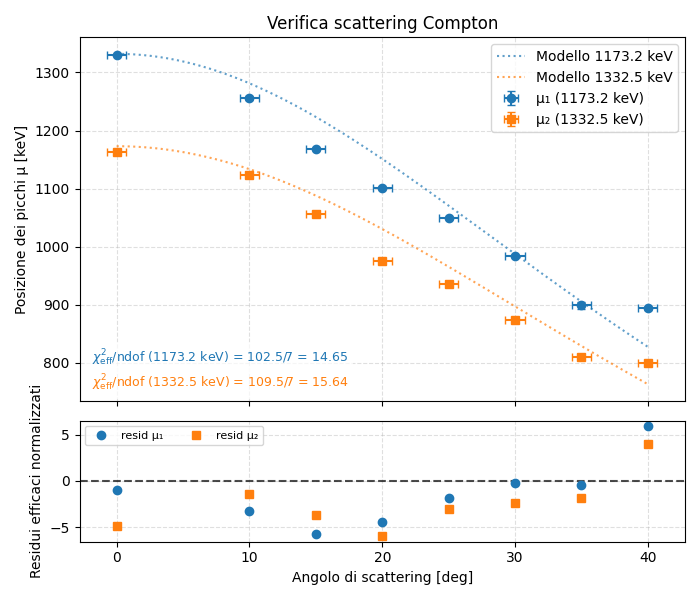
\includegraphics[width=0.9\linewidth]{verifica.png}
\centering
\caption{Confronto tra dati sperimentali e modello teorico. I residui e il valore di $\chi^2$ sono stati calcolati utilizzando la tecnica degli errori efficaci.}
\label{fig:verifica}
\end{figure}

Il valore del $\chi^2_{\text{eff}}/ndof$ calcolato per entrambe le curve risulta significativamente maggiore di 1:
\[
\left(\frac{\chi^2_{\text{eff}}}{ndof}\right)_1 = 14.65,
\qquad
\left(\frac{\chi^2_{\text{eff}}}{ndof}\right)_2 = 15.64.
\]

In accordo con quanto discusso in precedenza, tale discrepanza può essere attribuita principalmente a due contributi sistematici. Il primo è legato al fatto che, all'aumentare dell'angolo di scattering, la separazione energetica tra le due componenti del $^{60}$Co si riduce progressivamente, diventando comparabile o inferiore alla risoluzione energetica del rivelatore; oltre $20^\circ$ risulta quindi sempre più difficile distinguere i due picchi. Per ovviare a questa limitazione sarebbe necessario utilizzare una sorgente monocromatica, ad esempio $^{137}$Cs.

Il secondo contributo riguarda la calibrazione del rivelatore NaI(Tl), che può essere soggetta a errori sistematici tali da condurre a una sottostima della posizione dei picchi in energia.

Infine, le misure sono state effettuate nel corso di diverse ore. I punti di lavoro e il guadagno dei fotomoltiplicatori possono variare nel tempo, soprattutto a causa della loro sensibilità alle condizioni termiche ambientali. Questo effetto è particolarmente evidente nell'ultimo punto, relativo alla misura a $40^\circ$. A differenza delle altre configurazioni, acquisite in un'unica seduta di laboratorio della durata di $2$--$4$ ore, questa misura è durata circa $14$ ore ed è stata lasciata in acquisizione per un'intera notte. È quindi plausibile che variazioni di temperatura abbiano modificato il guadagno del fotomoltiplicatore, causando uno spostamento della posizione del picco. Questo ha complessivamente aumentato la varianza dei dati e reso tale punto il più distante dal modello teorico, nonostante l'elevata statistica raccolta.

Per mitigare questo problema, si potrebbe utilizzare una sorgente di calibrazione monocromatica in parallelo alla misura dello spettro del cobalto e, tramite un sistema di \textit{clock}, alternare l'acquisizione dei due spettri nel tempo. Sebbene ciò aumenterebbe significativamente la complessità del set-up sperimentale, permetterebbe di monitorare la calibrazione durante l'intera presa dati e, se necessario, ricalibrare ciascun punto individualmente anziché l'intera misura.


\section{Conclusioni}
In questa esperienza è stato possibile osservare sperimentalmente l’effetto Compton e verificare qualitativamente la relazione teorica che descrive la dipendenza dell’energia dei fotoni diffusi dall’angolo di scattering. L’andamento complessivo dei dati risulta compatibile con le previsioni del modello, confermando la validità del processo fisico descritto dalla formula di Compton.

L’analisi quantitativa mette tuttavia in evidenza una discrepanza sistematica tra dati e modello, come indicato dai valori elevati del $\chi^2_{\text{eff}}/ndof$. Tale comportamento è attribuibile principalmente alla difficoltà di risoluzione dei due picchi energetici del $^{60}$Co per angoli di scattering elevati, dove la separazione in energia diventa confrontabile con la risoluzione del rivelatore NaI(Tl), e a possibili errori sistematici nella calibrazione in energia. Ulteriori contributi possono derivare dalla variazione del guadagno dei fotomoltiplicatori durante acquisizioni di lunga durata, come osservato nella misura a $40^\circ$.

Nonostante queste limitazioni sperimentali, l’esperienza risulta complessivamente soddisfacente: il set-up ha permesso di evidenziare chiaramente il fenomeno dello scattering Compton e di discuterne in modo critico gli aspetti sperimentali e sistematici. Miglioramenti futuri potrebbero includere l’utilizzo di una sorgente monocromatica e un monitoraggio continuo della calibrazione, al fine di ridurre gli effetti sistematici e ottenere un confronto quantitativo più accurato con il modello teorico.

\onecolumn
\appendix
\section{Appendice: Simulazione Monte Carlo}
\label{app:MC}

Nel corso dell’esperienza è stata sviluppata una simulazione Monte Carlo con l’obiettivo di riprodurre la propagazione dei fotoni all’interno del set-up sperimentale e confrontarne i risultati con i dati acquisiti. La simulazione genera fotoni all’interno della sorgente e ne segue la propagazione nello spazio, includendo interazioni nel collimatore, nello scintillatore plastico e nel cristallo di NaI(Tl). Lo scopo principale è quello di studiare gli effetti geometrici e strumentali che influenzano lo spettro osservato sperimentalmente.

\subsection{La simulazione}

\subsubsection{Propagazione dei fotoni}

La simulazione procede per passi successivi: i fotoni vengono inizializzati sulla superficie di un materiale, propagati al suo interno (o nell’aria) e successivamente riportati sulla superficie esterna. Ad ogni passaggio, un fotone può essere assorbito completamente o uscire dal sistema attraverso superfici non rilevanti (ad esempio dal lato del collimatore); in tali casi il fotone viene rimosso dalla simulazione. Al termine di ogni passaggio, l’insieme dei fotoni sopravvissuti viene replicato in modo da mantenere costante la statistica totale.

A ciascun fotone è associato un peso, che rappresenta la probabilità che tale fotone contribuisca agli osservabili finali. Quando un fotone viene copiato, il suo peso viene opportunamente ridotto. All’interno dello scintillatore plastico i fotoni sono forzati a compiere uno scattering Compton; questa scelta, motivata da ragioni computazionali, evita di simulare e successivamente scartare un grande numero di fotoni che non interagiscono con il plastico. La distribuzione angolare dello scattering è determinata dalla sezione d’urto differenziale di Klein--Nishina

\begin{equation}
\frac{\mathrm{d}\sigma_{Compton}}{\mathrm{d}\cos\Phi} \propto 
\left(\frac{E'}{E_0}\right)^2 
\left(\frac{E'}{E_0} + \frac{E_0}{E'} - 1 + \cos^2\Phi\right),
\label{eq:KN}
\end{equation}

che viene normalizzata a distribuzione di probabilità e campionata in $\cos\Phi$ mediante \textit{reverse CDF sampling}. Poiché lo scattering è imposto artificialmente, il peso di ciascun fotone viene diviso per la probabilità di scatterare con l’angolo estratto. L’energia depositata nel plastico durante lo scattering Compton viene registrata e utilizzata successivamente nella modellizzazione delle soglie dei discriminatori.

Nel cristallo di NaI(Tl) viene simulata, in modo analogo, la competizione tra interazioni Compton e fotoelettriche. Un’interazione fotoelettrica deposita l’intera energia residua del fotone e ne causa la rimozione dalla simulazione, mentre dopo uno scattering Compton il fotone può continuare a propagare e interagire fino a uscire dal cristallo o essere assorbito. Le sezioni d’urto utilizzate sono state ricavate da tabelle sperimentali presenti in letteratura e permettono di descrivere l’interazione dei fotoni nel NaI(Tl) a qualsiasi energia.

\subsubsection{Modellizzazione della funzione di risposta del rivelatore}

Non avendo accesso diretto alla funzione di risposta dei rivelatori, è stato costruito un modello empirico per la risoluzione energetica $\sigma_E(E)$. Per ogni calibrazione giornaliera sono stati stimati sia il valore medio sia la varianza dei picchi energetici; assumendo le sorgenti come monocromatiche, la larghezza osservata dei picchi è stata attribuita alla risposta del cristallo. Ci si attende una dipendenza del tipo $\sigma_E(E) \propto \sqrt{E}$, per cui la risoluzione è stata modellizzata tramite una funzione quadratica

\[
\sigma_E^2(E) = aE^2 + bE + c,
\]

analogamente a quanto fatto per la calibrazione canale--energia in sezione \ref{subsec:calibrazione}. In questo modo, per ogni giornata di acquisizione è disponibile un modello della funzione di risposta del rivelatore NaI(Tl)\footnote{Durante le calibrazioni la sorgente è stata posta direttamente di fronte al rivelatore NaI(Tl), senza utilizzare il sistema di \textit{trigger} né lo scintillatore plastico}.  
Nel confronto tra simulazione e dati sperimentali, a ciascun evento simulato viene sommato un termine casuale estratto da una distribuzione gaussiana a media nulla e deviazione standard determinata dal modello di calibrazione del giorno corrispondente. Questo processo di \textit{smearing} simula l’effetto della risoluzione energetica del rivelatore.

\subsubsection{Modellizzazione delle soglie di discriminazione}

La simulazione descrive la geometria del set-up e i principali processi fisici, ma non include inizialmente l’effetto delle soglie dei discriminatori utilizzate sperimentalmente per ridurre il fondo e le coincidenze accidentali. Poiché tali soglie sono impostate in tensione e la loro funzione di risposta non è nota con precisione, esse sono state introdotte come parametri liberi del modello.

La simulazione restituisce, per ogni angolo, uno spettro pesato e un istogramma bidimensionale delle energie depositate nel plastico e nel cristallo, indicato come $H(E_{NaI}, E_C)$. La probabilità che un evento superi la soglia di un rivelatore è stata modellizzata mediante la funzione cumulativa di una distribuzione gaussiana

\begin{equation}
F(E;\mu,\sigma) = \frac{1}{2}\left[1 + \erf\left(\frac{E - \mu}{\sqrt{2}\sigma}\right)\right],
\label{eq:model_soglia}
\end{equation}

che rappresenta una soglia a gradino convoluta con una risposta gaussiana\footnote{La funzione di risposta del fotomoltiplicatore sul plastico è assunta gaussiana. Per il NaI(Tl), la risoluzione energetica è già stata modellizzata separatamente; la larghezza $\sigma$ associata alla soglia tiene conto esclusivamente delle fluttuazioni del discriminatore}.  

Il confronto con i dati sperimentali è stato effettuato tramite un fit di massimizzazione della likelihood utilizzando il modello

\begin{equation}
A \int H(E_{NaI}, E_C)\,
F(E_{NaI}; \mu_{NaI}, \sigma_{NaI})\,
F(E_C; \mu_C, \sigma_C)\,
\mathrm{d}E_C,
\label{eq:model_likelihood}
\end{equation}

dove $A$ è un parametro di normalizzazione. Il modello integra sulle energie depositate nel plastico e fornisce lo spettro simulato confrontabile direttamente con i dati.

\begin{figure*}[htp]
    \centering
    \begin{subfigure}[b]{0.3\textwidth}
        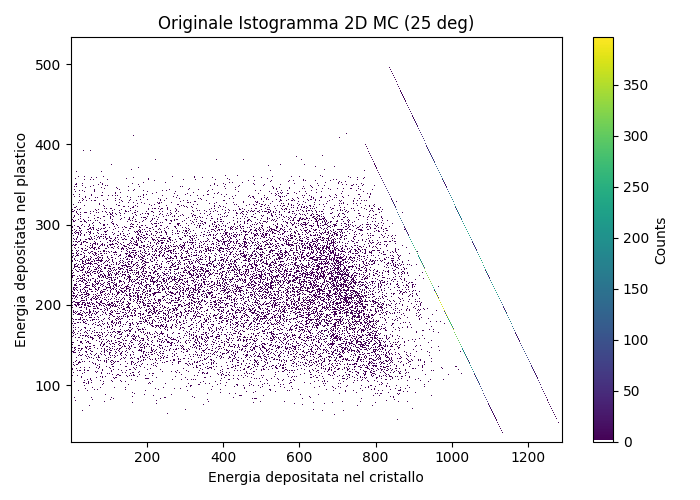
\includegraphics[width=\textwidth]{25degH.png}
        \caption{Istogramma bidimensionale delle energie depositate nei materiali}
    \end{subfigure}
    \hfill
    \begin{subfigure}[b]{0.3\textwidth}
        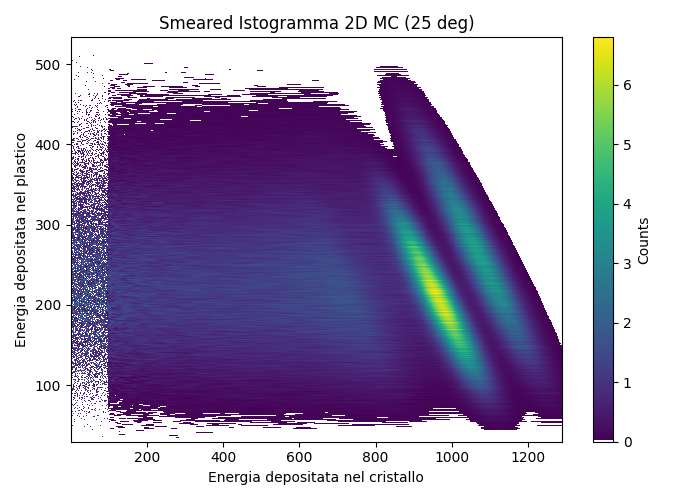
\includegraphics[width=\textwidth]{25degHS.png}
        \caption{Dati simulati dopo l’applicazione dello \textit{smearing} gaussiano}
    \end{subfigure}
    \hfill
    \begin{subfigure}[b]{0.3\textwidth}
        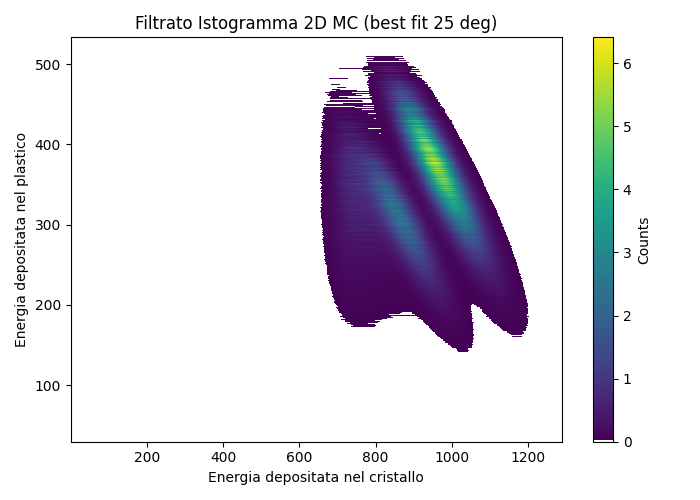
\includegraphics[width=\textwidth]{25degHF.png}
        \caption{Dati simulati filtrati dopo il fit con i dati sperimentali}
    \end{subfigure}
    \caption{Evoluzione degli istogrammi 2-D della simulazione a $25^\circ$}
    \label{fig:2dhists}
\end{figure*}

\subsection{Confronto con i dati sperimentali}

Il confronto tra simulazione Monte Carlo e dati sperimentali consente di valutare l’impatto delle soglie di discriminazione sulla forma dello spettro osservato. In particolare, la soglia sul NaI(Tl) riduce significativamente il fondo, mentre quella sullo scintillatore plastico limita la rivelazione dei fotoni più energetici, causando un restringimento dei picchi e l’eliminazione degli eventi ad energie più elevate.

In figura \ref{fig:25degfitted} è mostrato lo spettro simulato dopo l’applicazione del modello di soglia e l’integrazione sull’energia depositata nel plastico, a confronto con i dati sperimentali.

\begin{figure}[ht!]
\centering
\includegraphics[width=0.45\linewidth]{25degfitted.png}
\caption{Confronto tra dati sperimentali e simulazione Monte Carlo a $25^\circ$}
\label{fig:25degfitted}
\end{figure}

La simulazione riproduce qualitativamente la forma generale dello spettro; tuttavia, il fit restituisce valori delle soglie sul plastico significativamente più alti rispetto alle stime sperimentali (dell’ordine di \SI{100}{keV}) e valori di $\chi^2/ndof$ elevati ($\sim 2$--$10$). Ciò indica che la modellizzazione delle soglie non cattura completamente il comportamento reale del sistema.

Si conclude quindi che la simulazione Monte Carlo, pur includendo i principali effetti geometrici e fisici, non è in grado di descrivere in modo quantitativamente accurato tutti gli aspetti sperimentali. Nonostante ciò, l’esercizio si è rivelato utile per comprendere il ruolo delle soglie e della risposta dei rivelatori, e costituisce una base solida per eventuali sviluppi futuri della simulazione.

\end{document}
